% !TeX spellcheck = en_GB
\section{Experimental Set-up and Procedure}
\subsection{Set-Up}
The experiment was done with a pre mounted setup as shown in the fig \ref{fig:setup1} with tree main components: Laser source and optical components, electronic and microwave equipement and an Apparatus for NV centre spectroscopy. A reliable radio-frequency system must be deployed, ensuring the microwave-based excitation of the diamonds magnetic resonance. Its important that the osciloscope and the spectrum analizer need to be synchronized to achieve simultaneous optical analysis while sweeping the desired microwaves. a list of the apparatus used in this experiment and also pictures of the set up running can be find in the apendix.
\begin{figure}
	\centering
	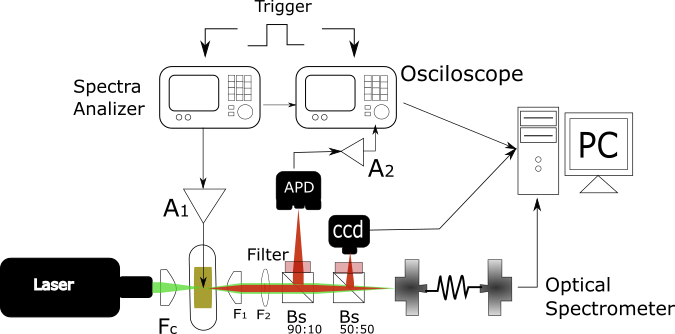
\includegraphics[width=0.7\linewidth]{../figures/setup1}
	\caption[setup]{Schematic not on scales of the experiment. The laser is coupled into an optical fiber and operated via software of Thorlabs. \textbf{Optics}: The laser is focussed on a microstrip (MS) with a condensor lens (Fc). Using a 4-f-system with the lenses f1 and f2 (having focal lengths of 10 and 80 mm, respectively) and a Beam splitting set;with split intensities 10:90 (beampath:APD), and 50:50 (CCD:OS), the diamonds are imaged on an avalanche photo diode (APD), the CCD-camera (CCD) and the optical spectrometer (OS). Low pass Color filters are addes to avoid the pass of the laser ligth.
	\textbf{Electronics}: The output of a spectrum analyzer is amplified (amplifier A1, gain = 48) and coupled into the microstrip, which is grounded through an impedance of 50Ω.
	The spectrum analyzer’s and the oscilloscope are triggered with the same signal, recording the signal of an power detector (ACDC), as well as the amplified signal (audio amplifier A2) of the APD.  Adapted from \cite{anleitung}.}
	\label{fig:setup1}
\end{figure}
 \subsubsection{Optical setup}
The optical compones basically conform a confocal microscope eith two lenses (f$1=10mm and f2=80mm$) set up at their focal points, forming a 4f-system. A laser of $\lambda=519nm$ was user as illumination source, In the set up an optic fiber had to be couple to the laser due lack of spacefocused with a condensor lend (fc).
In the object plane is the Microstrip \textbf{(Ms)}, in this objective we put a small portion of micro-diamonds powder with a small spire with out touchinf the strip. The Ms is fundamental to apply the ODMR measurements, a magnet holder is available, wich counts with a conector tp the spectra analizer \textbf{(DSa)} that supplies the microwaves.

An adjustable mirrors set provides ahelps to align the laser beam into the strip, givin 3 dimentions to move. For distribute the signal into the Avalanche PhotoDiode \textbf{(APD)} and the ccd camera Two dicroic mirros ( acting as beam spliater) was used, one with 90:10 porcent and 50:50 for the APD and the ccd andd optical spectrometer respectivelly. The advantage of using a APD is that it providing fast response in time and high sensitivity. ToensurethatmostoftheopticalpowerreachestheAPD, and that one is still able to perform spectroscopy and imaging at the same time. Both the CCD and spectrometer are controlled using a computer. To ensuavoid any scattered of ligth and improve a low signal-background ratio  low pass color filters \textbf{(CF)} was used after each beam spliter to avoid the laser ligth to be meassure in the data.

\subsubsection{Electronics}

Additionally to the optics, some electronics have to be addet to perform the ODMR.First an Osciloscope is used to read the APD signal after being amplified by an audio amplifies.  As mentioned, a supply of microwaves is couple to the MicroStrip.
Because the transition and reflection in the Ms is unknown an power coppler have to be add in the set up showe in the next section, so this trasmisson can be related directly.  To do so, a supply covering the frequency of center 2.8GHZ is used, which can be provided by the tracking generator of a spectrum analyzer (SA), it was set at odBm and conected to a 45dBm amplified before it reach the Ms as shown in \ref{fig:setup1}.
 A signal generator in square mode trigger the SA and the Osciloscope in order both meassuments coincides so the intensity of the flluorecence detected by the APD can be track imidiatly the microwaves was imput.
 
 Our tracking generator can sweep through the aforementioned range within 200ms, and  the signal generator was set to ......  Another way to increase the obtained signal is done on the acquisition site: an audio amplifier (A2) also increases the signal provided by the APD, which has previously been filtered using a low pass filter (cut-off frequency fc “100Hz). 
 
 The oscilloscope was used with a build-in phyton software already install in the computer ans sligthly modified just in the number of data adquire to 250loops per meassument......
 
 \subsubsection{Magnets}
 One the SA and the APD was trigered and the signal was well adquired, one and two magnets was add next to the Microstrip with the pourposse of allign the Diamond lattice with the magnetic field  and do some meassuments respecting this ne parameter.
two magnests was used, displayed in a base overpose to the Microstrid and centered to the diamonds powder. The distance between the magnets and the center was$36mm \pm 0.5$ and several variations was used, includin a perpenticular meassure in the Z axis and changing of  polarity.  In the next figure a sketchs of the base used is shown as the axis of the lab reference.
\begin{figure}
	\centering
	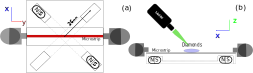
\includegraphics[width=0.7\linewidth]{../figures/magnets}
	\caption[mag]{top and side view of the magnet base over the microstrip, The magnets was put in the strips of the base alwasys at the same distance, the reference of the axis are respective the laboratory frame.}
	\label{fig:magnets}
\end{figure}


\subsection{Calibration}
\subsubsection{convertion factor camera}
The strip was meassure with a calibrator at $1.2\pm 0.1\,\mathrm{mm}$ and the camara used was a Thorlabs CCD camera with dimentions of 1280x1024 pixels, each pixel with $5.2\times5.2 \mathrm{\mu m}$ according to the manufacturer.
In order to know the actual resolution of our microscope a calibration was done based on the magnification and calibration factor of the set up.
Theoritically our $C_{f}$ can be calculated as:
\\

\begin{equation}
C_{f}=\dfrac{1 px \cdot M}{d_{p}} = 1552 px/mm
\end{equation}\\
Where $M$ is the magnification and $d_{p}$ is the pixel sizes. And with a Magnification icual to the lenses used for the confocal setup is equal to the magnification $M=f2/f1=8$.
In this case the tool of Thorlab’s software was used to determine and measure the width of the microstrip. Using the equation above and the respective measumente we denote that  $C_{f} =1346 \,\mathrm{px/mm}$, with a magnification factor close to $M=7X$.

\subsubsection{Laser Power}
To set the power of the laser to a reasonable value a calibration curve was recorded which shows the actual laser power at the position of the microstrip plotted over the output power set in the GUI. This curve is shown in figure \ref{fig:power}.\\

Using this graph the output power was set to $P_\text{out}=20\,\mathrm{mW}$ which corresponds to an actual laser power of $P_\text{act}=(27.4\pm1.4)\,\mathrm{mW}$.
\begin{figure}[hb]
	\centering
	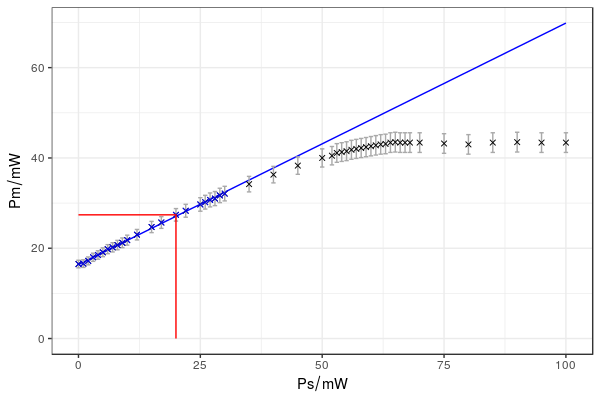
\includegraphics[width=\textwidth]{../figures/powercal.png}
	\caption{Measurement of the laser power}
	\label{fig:power}
\end{figure}


\subsubsection{Electronic components}

In order Performe our ODMR, is crucial to determine the amount of microwave power deployed into the microstrip and the diamonds. we can not have an absolut power that is been pluging into the set up. The microstrip by defoult have some transmition $T_{Ms}$ and reflecctions $R_{Ms}$ that are unkown.
For this a power coupler was added to the setup and four meassument with diferents arranges where performed as shown in the fig...
First, the power coupler was conected to the DSA in out- out possition to knoe the transmitio of it, $T_{cpl}$. on the other hand the secon setup is an Out conection to the DSA and help to determine the reflection of the CPL $R_{cpl}$. for the thirt and fouth display, the mmicrostrip was added, in the Out-Out possition ( CPL-DSA), messurion the Reflection $R_{cpl-Ms}$ and transmition $T_{cpl-Ms}$ of the hole set.

\begin{figure}
	\centering
	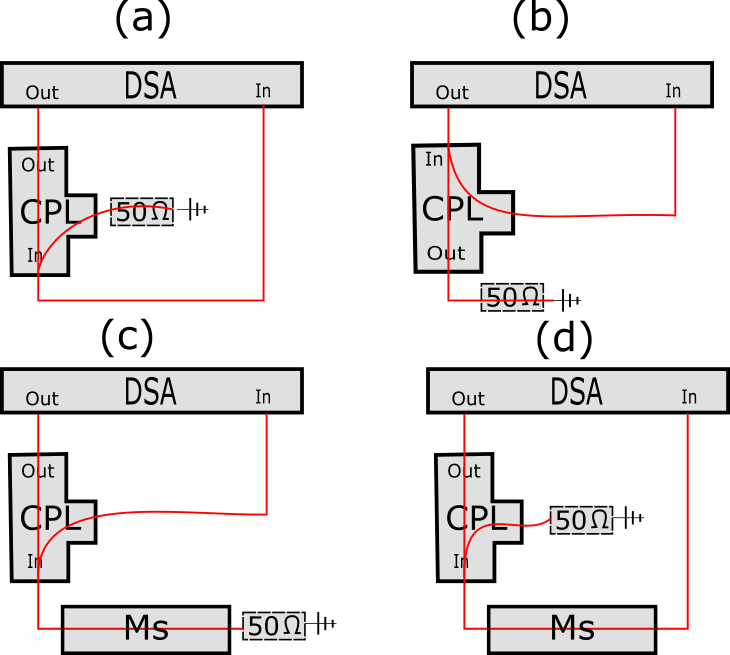
\includegraphics[width=0.7\linewidth]{../figures/APD}
	\caption[diferent arranges of the CPL and MicroStrip conected to the DSA]{(A) CPL conected to the DSA in Out-Out direction messuring $T_{cpl}$, (b) Cpl conected in Out-In secuence and meassuring $R_{cpl}$, (c) CPl and microstrip conected in Out-Out mode and measuring the $R_{cpl-Ms}$ (d) CPL and Microstrip conected in Out-Out moded and meassuring $T_{cpl-Ms}$}
	\label{fig:apd}
\end{figure}

The DSA was set at 0 Dbm and a sweep centered at 2.8GHz frequancy. A 50$\Omega$ resistance was used for the losses ends as shown. The next figure display the four signals of the diferent arranges.
\begin{figure}
	\centering
	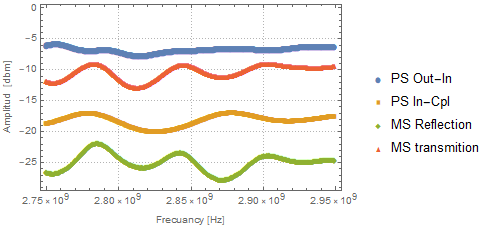
\includegraphics[width=0.7\linewidth]{../figures/microstrip}
	\caption{Atenuattion od the power at 0dBm from top to bottom: $T_{CPL}$,$T_{Cpl-Ms}$, $R_{CPL}$ and $R_{Cpl-MS}$}
	\label{fig:microstrip}
	\end{figure}

The total transmition and reflection ws simply calculated by a sustraction of the Ms trasmition in the diferent processes as next.

\begin{align}
T_{Ms}&=T_{cpl-Ms}-T_{cpl}\\
R_{MS}&=R_{cpl-Ms}+T_{cpl}-R_{cpl}
\end{align}


The attenuation in this cases for the transmission remains close to cero, specially in the center of the sweep while the reflection as shown reduces drasticly. This gives  us the facts that the power transmitted is close to the 0dBm used in the DSA and few of it is been reflected.

\begin{figure}
	\centering
	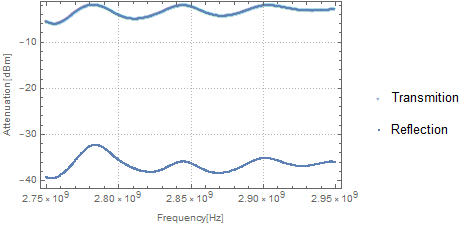
\includegraphics[width=0.7\linewidth]{../figures/microstrip-trasm-eflect}
	\caption[trans-refl]{Ateniation of the resultant transmition (top) and reflectrion (bottom) at the Micristrip, at 0dBm in a 2.8GHZ frequency center.}
	\label{fig:microstrip-trasm-eflect}
\end{figure}

\subsubsection{Optical Spectrometer}
The optical spectrometer is later used to record the fluorescence spectrum of the diamond. To calibrate the optical spectrometer we first record the spectrum of visible light and compare the identified Fraunhofer lines with their literature values. The recorded spectrum is shown in figure \ref{fig:sunspectrum} and the values are given in table \ref{tab:fraunhofer}.\\

Since only small statistical deviations in both directions could be found there was no need to calculate a conversion factor and the values given from the optical spectrometer were verified. \\

The optical spectrometer was also used to get the actual wavelength of the laser which was determined in figure \ref{fig:laserspectrum} to be $\lambda=(517.3\pm0.2)\,\mathrm{nm}$.
\begin{figure}
	\centering
	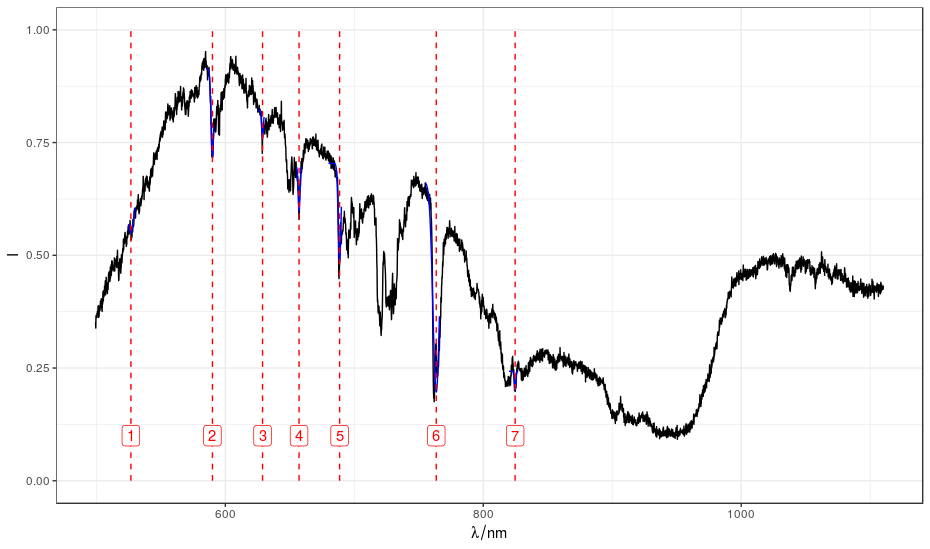
\includegraphics[width=0.8\textwidth]{../figures/sunspectrum.png}
	\caption[Spectrum of the sun with identified Fraunhofer lines]{Spectrum of the sun with identified Fraunhofer lines for calibration of the optical spectrometer}
	\label{fig:sunspectrum}
\end{figure}

\begin{table}
	\centering
	\begin{tabular}{c|c|c|c|c}
		Peak&Position&Element&Position \cite{fraunhoferlines}&Difference\\
		1&$526.8\pm1.7$&Fe I&527.0&$-0.2$\\
		2&$590.0\pm0.5$&Na I&589.6&$+0.4$\\
		3&$628.9\pm0.3$&Fe I&630.3&$-1.4$\\
		4&$657.2\pm0.3$&H $\alpha$&656.3&$+0.9$\\
		5&$688.6\pm0.5$&&&\\
		6&$763.5\pm1.3$&&&\\
		7&$824.7\pm0.3$&&&\\
	\end{tabular}
	\caption{Positions of the Fraunhofer Lines compared to the literature values}
	\label{tab:fraunhofer}
\end{table}

\begin{figure}
	\centering
	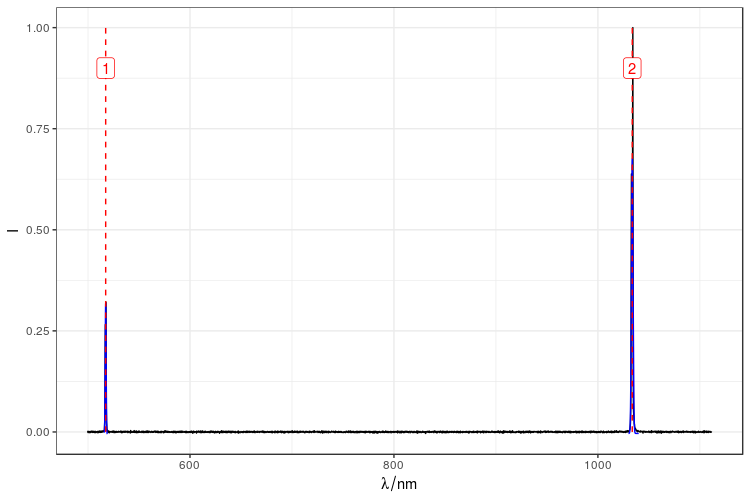
\includegraphics[width=0.8\textwidth]{../figures/laserspectrum.png}
	\caption[Spectrum of the laser]{Spectrum of the laser with identified peaks at the wavelengths $\lambda=(517.3\pm0.2)\,\mathrm{nm}$ and $\lambda=(1033.7\pm0.4)\,\mathrm{nm}$}
	\label{fig:laserspectrum}
\end{figure}

\subsubsection{ODMR calibrations}
\paragraph{Shielding}
To improve the ODMR signal and avoid noise generated by the microwaves a shielding cage was built around the APD. In figure \ref{fig:odmr-shield} the effect of this shielding cage on the ODMR spectrum is shown.
\begin{figure}
	\begin{subfigure}{0.5\textwidth}
		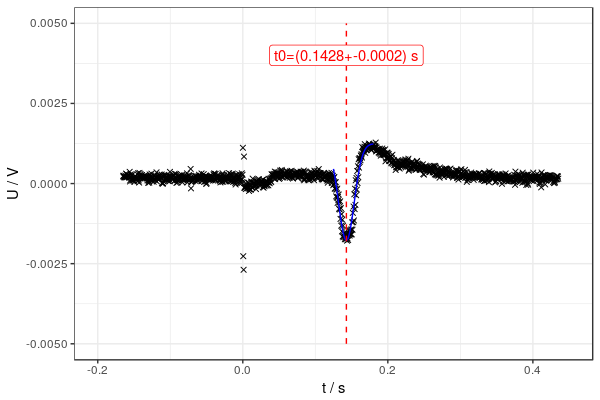
\includegraphics[width=\textwidth]{../figures/odmr-cal-1.png}
		\subcaption{without shielding}
	\end{subfigure}
	\begin{subfigure}{0.5\textwidth}	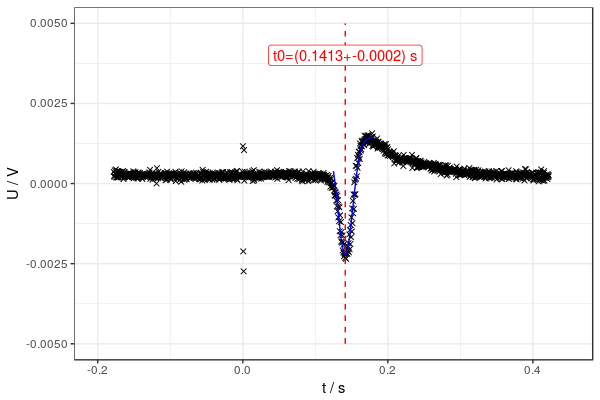
\includegraphics[width=\textwidth]{../figures/odmr-cal-2.png}
		\subcaption{with shielding}
	\end{subfigure}
	\caption{ODMR spectrum}
	\label{fig:odmr-shield}
\end{figure}
\paragraph{Time-to-Frequency Conversion}

\begin{figure}
	\begin{subfigure}{0.5\textwidth}
		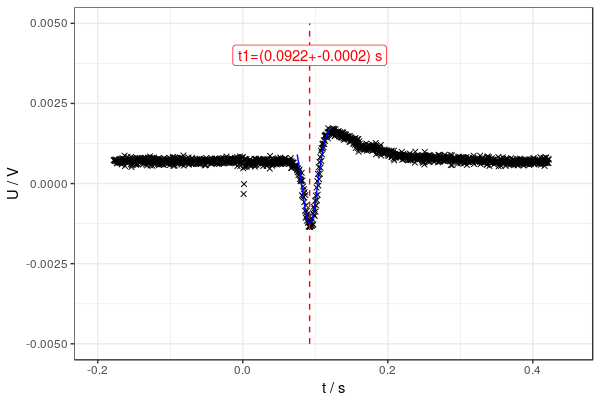
\includegraphics[width=\textwidth]{../figures/odmr-cal-4.png}
		\subcaption{shifted to the left}
	\end{subfigure}
	\begin{subfigure}{0.5\textwidth}
		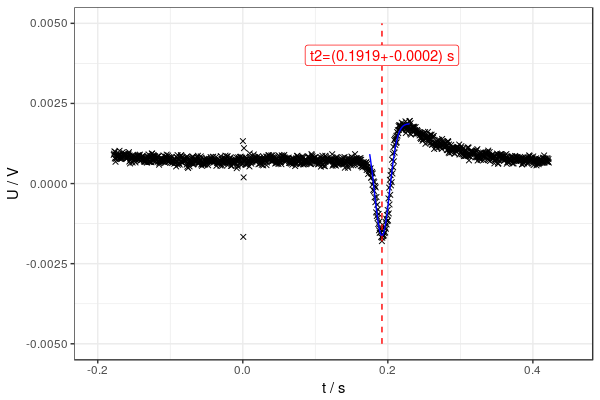
\includegraphics[width=\textwidth]{../figures/odmr-cal-3.png}
		\subcaption{shifted to the right}
	\end{subfigure}
	\caption{ODMR spectrum for time-to-frequency calibration}
	\label{fig:odmr-shift}
\end{figure}

Performing ODMR measurements we achieve the ODMR spectra on the oscilloscope. Therefore the spectra are time-resolved. To gain frequency-resolved spectra we need to calculate the conversion factor from time to frequency. We do this by performing two sweeps with shifted centre frequencies which allows us to calculate the conversion factor and also the offset since we know the frequency at which the peak appears.

The conversion can be expressed by the following equation:

\begin{align}
f(t)&=\frac{f(t_1)(t_1-t_2)-(f(t_1)-f(t_2))t_1}{t_1-t_2}+\frac{f(t_1)-f(t_2)}{t_1-t_2}\cdot t
\end{align}

Inserting the values achieved from figure \ref{fig:odmr-shift} we get the following conversion function:

\begin{align}
f(t)&=(1.003\pm0.003)\,\mathrm{\frac{GHz}{s}}\cdot t+(2.728\pm0.011)\,\mathrm{GHz}
\end{align}

Later in this document all spectra are converted by this function and therefore shown in the frequency domain. The errors are gained from the fit and propagated using Gaussian error propagation.

\subsection{Measurements}